\chapter{Estado de Arte}
\label{sec:estado-arte}

Neste capítulo será feita uma análise de algumas plataformas existentes para recolha de dados em estratégias de inbound marketing. A recolha de informação nos dias de hoje tem um grande impacto na forma como os negócios são feitos, principalmente na internet. Neste contexto, serão analisadas algumas das soluções que partilham funcionalidades semelhantes com o que vai ser desenvolvido.\\
Como referido no capítulo anterior, o modelo de negócio da plataforma é \gls{b2b} e neste sentido as caracteristicas analisadas serão focadas na segmentação de dados, integração com serviços externos, planos de pagamento e funcionalidades do \textit{back office}.
Seguindo uma das estratégias de inbound marketing, o método de envio de formações e recolha de dados será através da formulários online e por isso mesmo algumas características associadas à experiencia do utilizador, como por exemplo a personalização do formulário, serão também analisadas.


As plataformas a analisar serão o SurveyMonkey\cite{surveymonkey}

Após a apresentação destas ferramentas será feita uma análise das vantagens e desvantagens de cada uma, assim como a comparação de funcionalidades.


\section{SurveyMonkey}
\label{surveyMonkey}

O SurveyMonkey é um \acrfull{saas} de criação de questionários online. É necessário criar conta para aceder às funcionalidades da plataforma, dando a opção de utilizar serviços externos para esse efeito (e. g. Facebook\cite{face}, LinkedIn\cite{linkedin}), como podemos ver na Figura \ref{fig:surveymonkey_singin}.

\begin{figure}[ht!]
	\begin{center}
		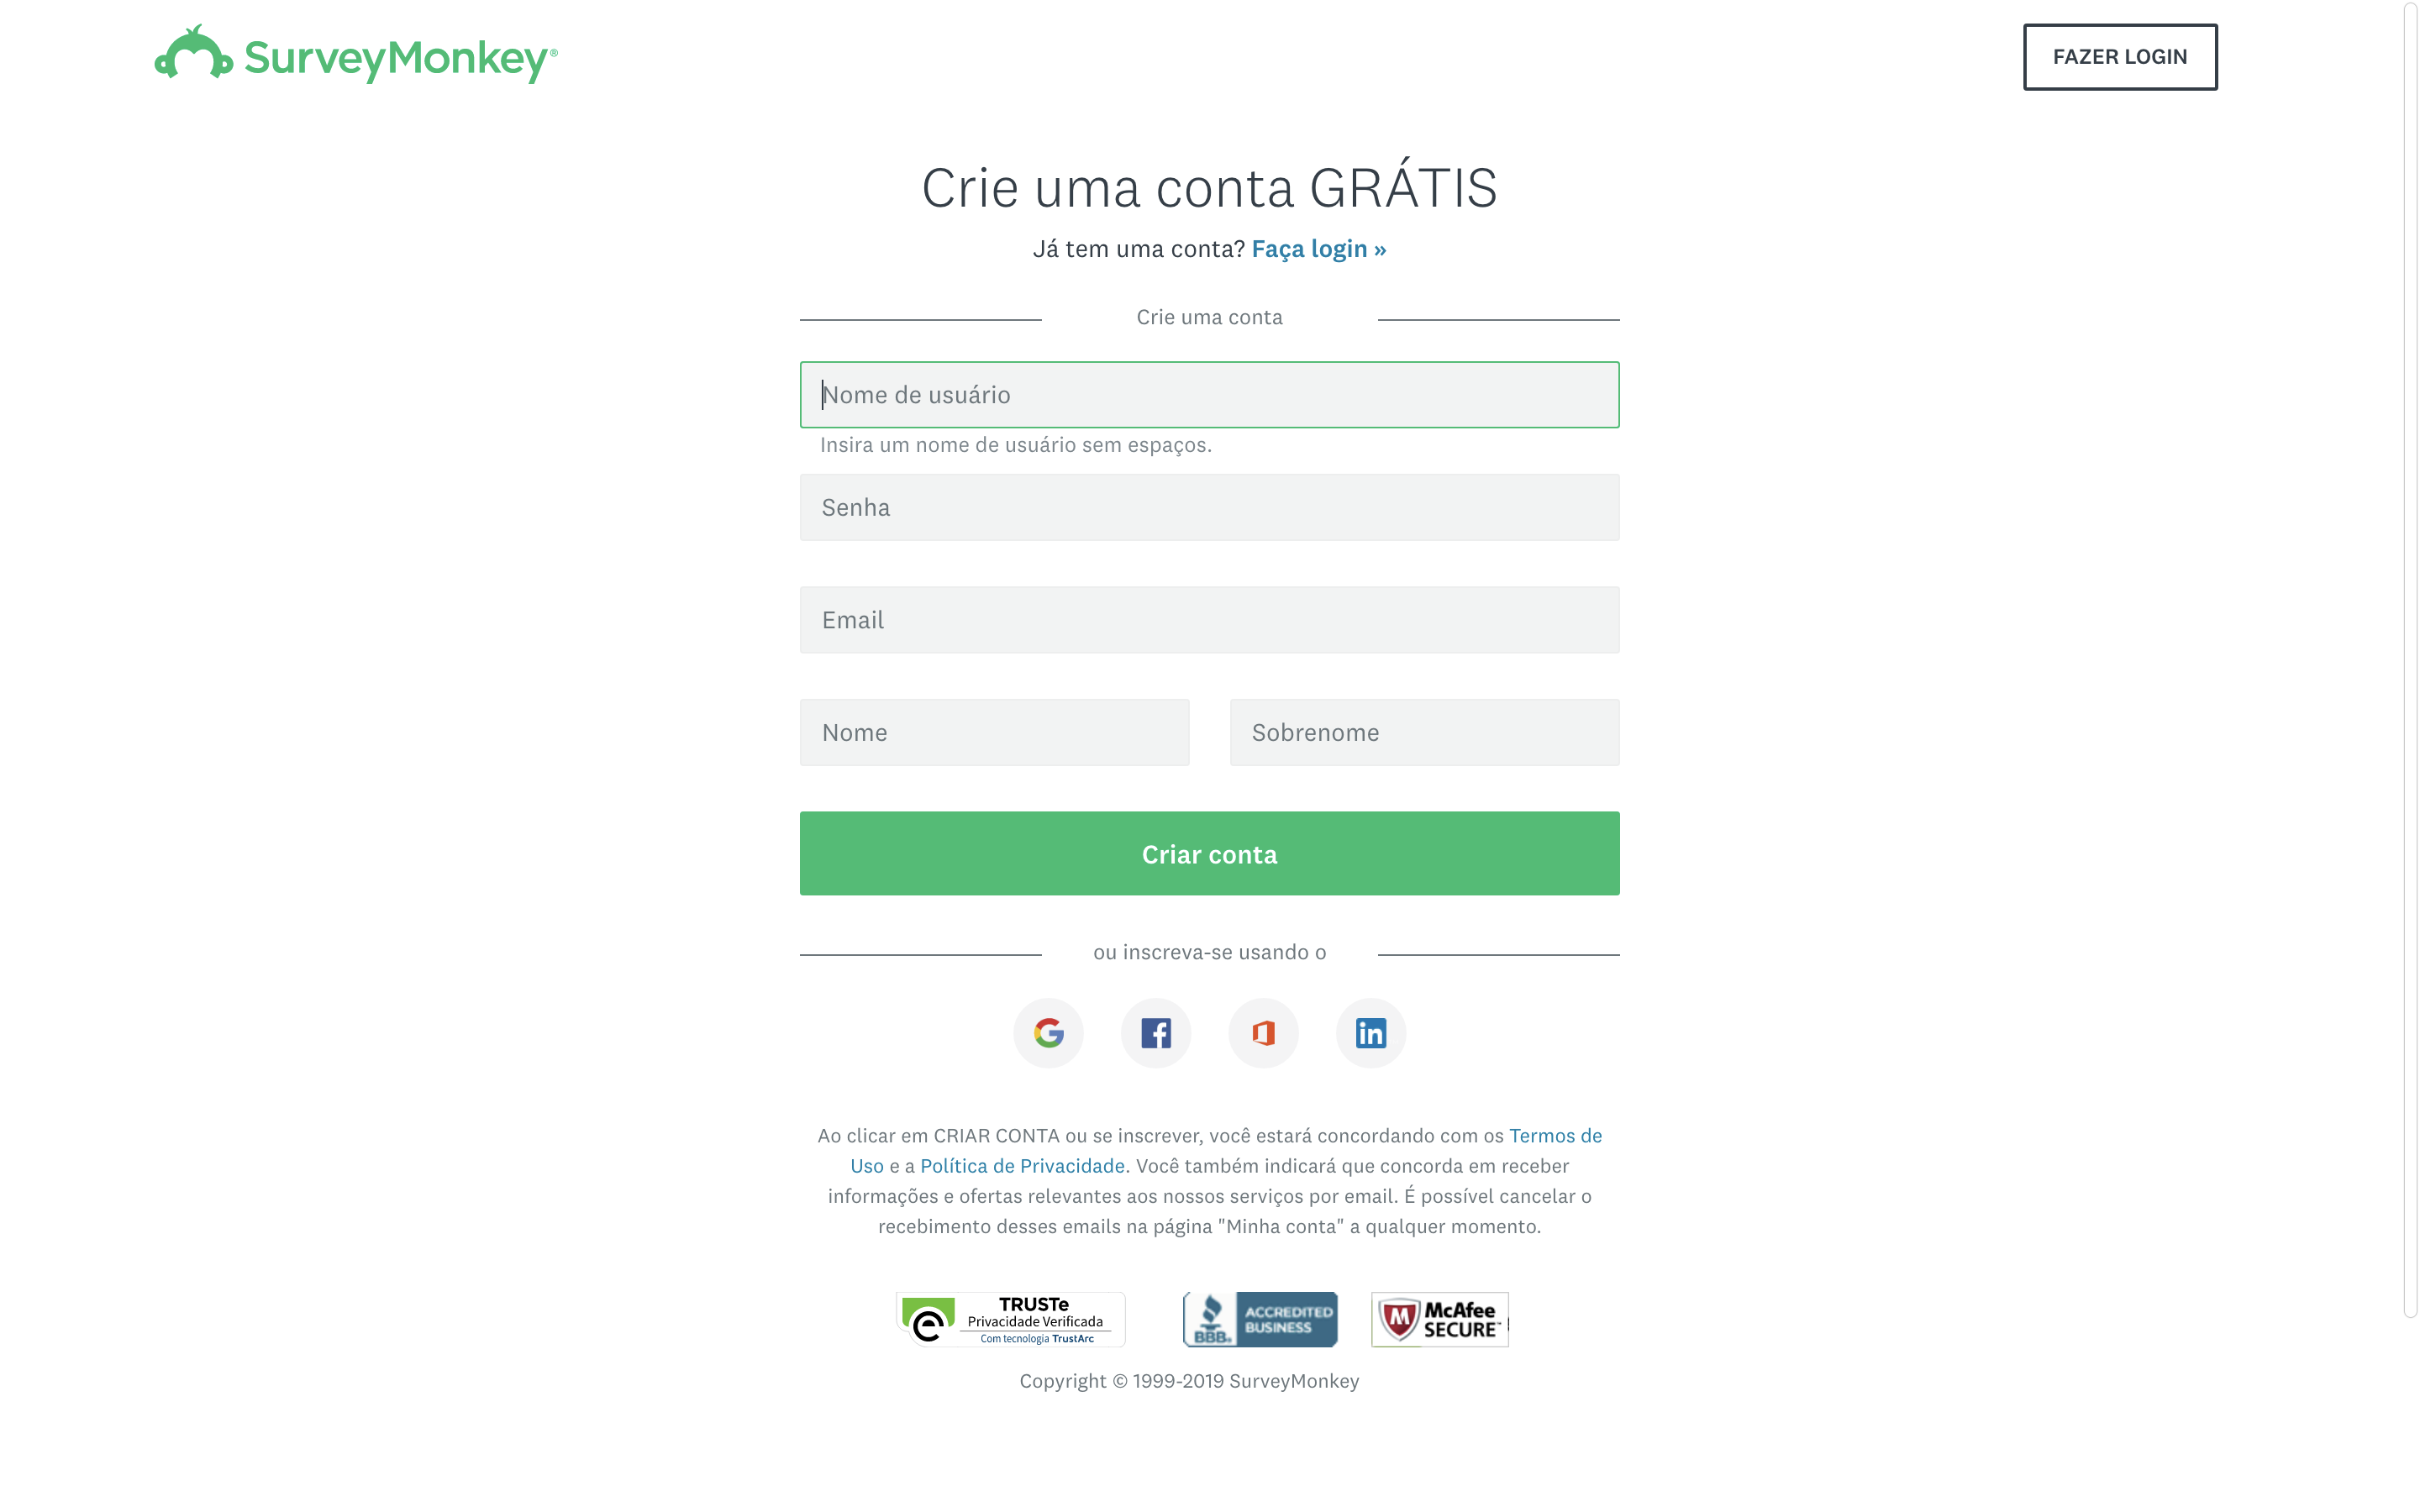
\includegraphics[width=1\textwidth]{img/surveymonkey-singin}
		\caption{SurveyMonkey - Registro }
		\label{fig:surveymonkey_singin}
	\end{center}
\end{figure}

\newpage


sdfsdfsdf

%-------------------------------------------------------------------------------------------------
\blankpage
%-------------------------------------------------------------------------------------------------

\glsresetall



